\chapter{Results}
In this chapter our 

\section{Graph Database}
% Power of graph databases
We are dealing with connected data, where choosing a graph database have two advantages according to \citet{robinson2013}: performance and flexibility. In a relational database, the join-intensive query performance deteriorates as the dataset gets larger while, with a graph database the performance remains relatively constant. This is due to the fact that a query is only localized to a fraction of the graph making the run time proportional to the size of the sub-graph related to the query rather than the overall graph containing all available data.

Furthermore, there is the aspect of flexibility. Graphs are naturally additive \cite{robinson2013} such that new sub-graphs can be added containing more nodes and edges and new relations can be introduced as the understanding of the dataset grows. This have a positive implication for the analysts that does not have to model the domain in exhaustive detail from the start but can add information as time progress. 

Thus, according to the motivation above, we expect to use Neo4j, which is a cloud based graph database supporting some basic analysis through their query language Cypher.

\section{Gh0st RAT}
% In discussion - what similarity measure was the most appropriate to use in our case?

\begin{figure}[h!]
    \centering
    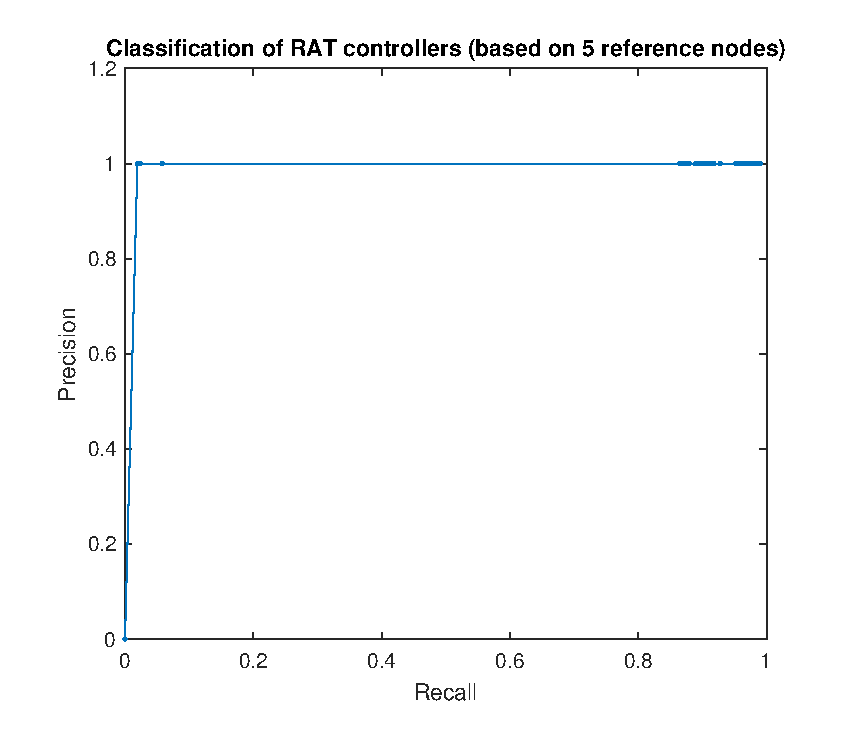
\includegraphics[width=0.4\textwidth]{precisionRecallRAT.eps}
    \caption{Caption}
    \label{fig:my_label}
\end{figure}

\begin{figure}[h!]
    \centering
    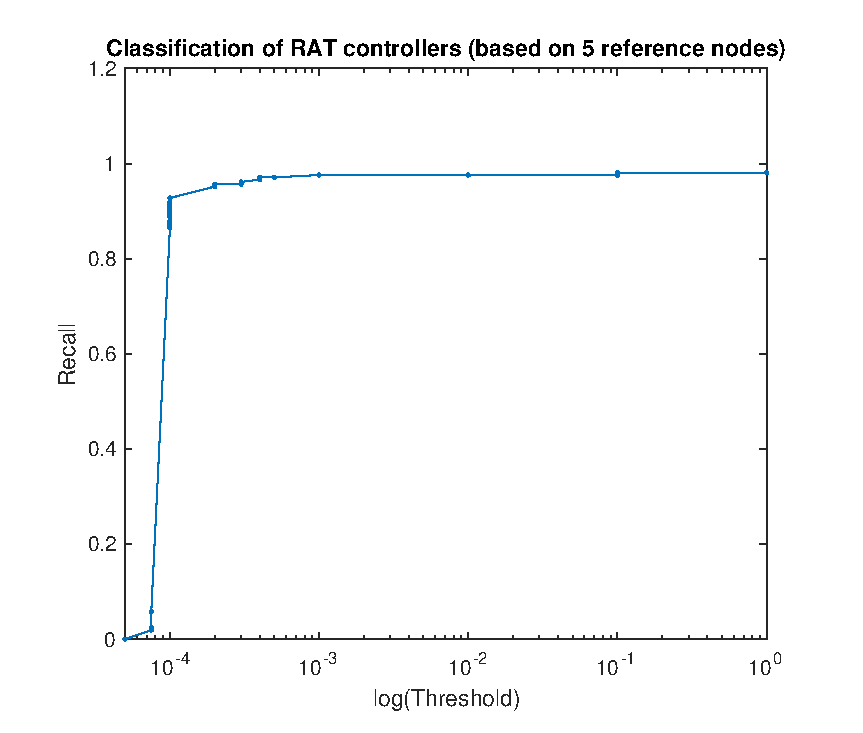
\includegraphics[width=0.4\textwidth]{recallThresholdRAT.eps}
    \caption{Caption}
    \label{fig:my_label}
\end{figure}

\section{Classification of malicious IP addresses}

\section{Redundancies}

\section{Target and Attackers}





\begin{comment}
\section{Multidimensional graph}
We expect a data representation where we have a multipartitioned graph, meaning there is a number of different nodes representing different kinds of entities with multiple edges, representing different relations, in between the nodes. Hence, we will then obtain a multidimensional network. 

\section{Analysis}
As far as the analysis goes, we expect to perform clustering to identify communities and link analysis to find different paths between two nodes. The latter can easily be queried in Neo4j and is expected to contribute a great deal solving the different questions. We also expect to use of some statistical tools such as average node degree, degree distribution and network diameter.
\end{comment}